
% ----------------------------------------------------------------------
%  Set the document class
% ----------------------------------------------------------------------
\documentclass[11pt,a4paper,twoside]{article}

% ----------------------------------------------------------------------
% Define external packages, language, margins, fonts and new commands
% ----------------------------------------------------------------------
%\input{preamble} 
\usepackage[utf8]{inputenc}   % <<<<< Linux
\usepackage[english]{babel} % <<<<< English
\usepackage{notoccite}
\usepackage[skip=0.5\baselineskip]{caption}
\hyphenation{GTKWave}
\usepackage{listings}
\usepackage[all]{nowidow}

%blind text
\usepackage{lipsum}

\usepackage{comment} % comment out large bodies of text

\usepackage{graphicx}
\graphicspath{ {./} {../../figlib/} }
\def\FontLn{% 16 pt normal
  \usefont{T1}{phv}{m}{n}\fontsize{16pt}{16pt}\selectfont}
\def\FontLb{% 16 pt bold
  \usefont{T1}{phv}{b}{n}\fontsize{16pt}{16pt}\selectfont}
\def\FontMn{% 14 pt normal
  \usefont{T1}{phv}{m}{n}\fontsize{14pt}{14pt}\selectfont}
\def\FontMb{% 14 pt bold
  \usefont{T1}{phv}{b}{n}\fontsize{14pt}{14pt}\selectfont}
\def\FontSn{% 12 pt normal
  \usefont{T1}{phv}{m}{n}\fontsize{12pt}{12pt}\selectfont}

% Use Arial font as default
%
\renewcommand{\rmdefault}{phv}
\renewcommand{\sfdefault}{phv}
\usepackage{geometry}	
\geometry{verbose,tmargin=2.5cm,bmargin=2.5cm,lmargin=2.5cm,rmargin=2.5cm}

%\usepackage{setspace}
%\renewcommand{\baselinestretch}{1.5}

\usepackage[pdftex]{hyperref} % enhance documents that are to be
                              % output as HTML and PDF
\hypersetup{colorlinks,       % color text of links and anchors,
                              % eliminates borders around links
%            linkcolor=red,    % color for normal internal links
            linkcolor=black,  % color for normal internal links
            anchorcolor=black,% color for anchor text
%            citecolor=green,  % color for bibliographical citations
            citecolor=black,  % color for bibliographical citations
%            filecolor=magenta,% color for URLs which open local files
            filecolor=black,  % color for URLs which open local files
%            menucolor=red,    % color for Acrobat menu items
            menucolor=black,  % color for Acrobat menu items
%            pagecolor=red,    % color for links to other pages
            pagecolor=black,  % color for links to other pages
%            urlcolor=cyan,    % color for linked URLs
            urlcolor=black,   % color for linked URLs
	          bookmarks=true,         % create PDF bookmarks
	          bookmarksopen=false,    % don't expand bookmarks
	          bookmarksnumbered=true, % number bookmarks
	          pdftitle={report},
            pdfauthor={Conanga, H.P.},
%            pdfsubject={Thesis Title},
%            pdfkeywords={Thesis Keywords},
            pdfstartview=FitV,
            pdfdisplaydoctitle=true}

\usepackage[numbers,sort&compress]{natbib} % <<<<< References in numbered list [1],[2],...
\usepackage{subcaption} 
\usepackage{mdframed}
\usepackage{amsmath} % facilitates writing math formulas and improves the typographical quality of their output
\setcounter{MaxMatrixCols}{20} % enables latex to make matrices w/ 20 columns


%%%%%%%%%%%%%%%%%%%%%%%%%%%%%%%%%%%%%%%%%%%%%%%%%%%%%%%%%%%%%%%%%%%%%%%%
%     Begin Document                                                   %
%%%%%%%%%%%%%%%%%%%%%%%%%%%%%%%%%%%%%%%%%%%%%%%%%%%%%%%%%%%%%%%%%%%%%%%%


\begin{document}

% Set plain page style (no headers, footer with centered page number)
\pagestyle{plain}

% Set roman numbering (i,ii,...) before the start of chapters
%\pagenumbering{roman}

% ----------------------------------------------------------------------
%  Cover page
% ----------------------------------------------------------------------
%%%%%%%%%%%%%%%%%%%%%%%%%%%%%%%%%%%%%%%%%%%%%%%%%%%%%%%%%%%%%%%%%%%%%%%%
%                                                                      %
%     File: Thesis_FrontCover.tex                                      %
%     Tex Master: Thesis.tex                                           %
%                                                                      %
%     Author: Andre C. Marta                                           %
%     Last modified :  2 Jul 2015                                      %
%                                                                      %
%%%%%%%%%%%%%%%%%%%%%%%%%%%%%%%%%%%%%%%%%%%%%%%%%%%%%%%%%%%%%%%%%%%%%%%%

\thispagestyle {empty}

% IST Logo - Signature A
% parameters: bb=llx lly urx ury (bounding box), width=h_length, height=v_length, angle=angle, scale=factor, clip=true/false, draft=true/false. 
%\includegraphics[bb=9.5cm 11cm 0cm 0cm,scale=0.29]{IST_A_CMYK_POS}

\begin{center}
%
% Figure (Image or plot)
\vspace{1.0cm}
% height = 50 mm
%\includegraphics[height=50mm]{Figures/Airbus_A350.jpg}

% Title, author and degree
\vspace{1cm}
{\FontLb Circuit Theory and Electronics Fundamentals} \\ % <<<<< EDIT TITLE
\vspace{1cm}
{\FontSn BSc Aerospace Engineering, Técnico, University of Lisbon} \\ % <<<<< EDIT COURSE
\vspace{1cm}
{\FontSn Lab 1: Circuit analysis methods} \\
\vspace{1cm}
{\FontSn March 25, 2021} \\ % <<<<< EDIT DATE (corresponds to date of oral examination)
\vspace{1cm}
{\FontSn Group 48} \\ %group
{\FontSn Dinis Papinha, 84379} \\ %authors
{\FontSn Filipa Gonçalves, 89662} \\ %authors
{\FontSn Carlos de Vasconcelos, 90227} \\ %authors
%
\end{center}


% ----------------------------------------------------------------------
% Dedication page (optional)
% ----------------------------------------------------------------------
%\input{dedication} 
%\cleardoublepage

% ----------------------------------------------------------------------
%  Acknowledgments (optional)
% ----------------------------------------------------------------------
%\input{acknowledgements}
%\cleardoublepage

% ----------------------------------------------------------------------
%  Abstract (both in English and Portuguese)
% ----------------------------------------------------------------------
%\input{resumo} 
%\cleardoublepage

%\input{abstract} 

% ----------------------------------------------------------------------
%  Table of contents, list of tables, list of figures and nomenclature
% ----------------------------------------------------------------------

% Table of contents
%
\tableofcontents

% List of tables
%\addcontentsline{toc}{section}{\listtablename}
%\listoftables
%\cleardoublepage 

% List of figures
%\addcontentsline{toc}{section}{\listfigurename}
%\listoffigures
%\cleardoublepage 

% Set arabic numbering (1,2,...) after preface
%
%\setcounter{page}{1}
%\pagenumbering{arabic}

% ----------------------------------------------------------------------
%  Body
% ----------------------------------------------------------------------

\section{Introduction}
\label{sec:introduction}

% state the learning objective 
The objective of this laboratory assignment is to study a circuit containing a
sinusoidal voltage source $V_I$ connected to a resistor $R$ and a capacitor $C$
in series. The circuit can be seen if Figure~\ref{fig:rc}.



\section{Theoretical Analysis}
\label{sec:analysis}

\subsection{Node Method}
\label{subsec:node}


The circuit consists of 8 nodes: 0 (ground), 1, 2, 3, 5, 6, 7 and 8, respectively associated with nodal voltages $V_0$, $V_1$, $V_2$, $V_3$, $V_5$, $V_6$, $V_7$ and $V_8$ (seen in Figure~\ref{fig:OG_circ}). 

% O que está para baixo

Because we are considering a DC voltage source, there is no current variation, hence the current $I_c=0$, so its consideres as being an open circuit between $V_6$ and $V_8$.

By first looking at the circuit we can assume the following equalities:


\begin{equation}
  V_1=V_s
  \label{eq:N_1}
\end{equation}


\begin{equation}
    I_c=0
    \label{eq:aux}
\end{equation}


\begin{equation}
    K_b\cdot V_b - I_b =0
    \label{eq:aux1}
\end{equation}


\begin{equation}
    -V_c + K_d \cdot I_d=0
    \label{eq:aux2}
\end{equation}


\begin{equation}
    -V_b + V_2 - V_5 = 0
    \label{}
\end{equation}

 \begin{equation}
     (V_5-V_8) + V_d=0
 \end{equation}




%\Using Ohm's Law

The other equations needed to solve this problem can be achived with Kirchoff's Current Law (KCL) and Ohm's Law:

\textit{Supernode 1}
\begin{equation}
    G_1 \cdot (V_1 - V_2) + G_4 \cdot V_5 +I_d=0
 \end{equation}
 


\textit{Node 2}
\begin{equation}
    G_1 \cdot (V_2 - V_1) + G_2 \cdot (V_2 - V_3) + G_3 \cdot(V_2 -V_5)=0
\end{equation}

\textit{Node 3}
\begin{equation}
    G_2 \cdot (V_3 - V_2) + K_b \cdot (V_5 - V_2)=0
\end{equation}

\textit{Node 6}
\begin{equation}
    K_b \cdot (V_2 - V_5) + G_5 \cdot (V_6-V_5)=0
\end{equation}

\textit{Node 7}
\begin{equation}
    G_7 \cdot(V_7 - V_8) + G_6\cdot V_7=0
\end{equation}


% O que está para cima, 

In order to obtain the currents running through branches formed by resistors, Ohm's law is applied. Furthermore, given that this is yet a DC circuit and assuming its in a stationary state (a lot of time has passed and the capacitor is fully charged), there is no current in the capacitor's branch. All the other branches are formed by sources and all of them are associated with one node that is "connected" to only one other branch, of which the current is known (they are resistor branches). Hence, applying KCL to these ("in common") nodes, the last unknown currents are obtained.

In octave we get the values present in Tabel \ref{tab:op}


\begin{table}[h]
  \centering
  \begin{tabular}{|l|r|}
    \hline    
    {\bf Name} & {\bf Value [A or V]} \\ \hline
    \input{teorico1}
  \end{tabular}
  \caption{Values for the components using the node method.}
  \label{tab:op}
\end{table}



\subsection{Equivalent Resistance}
\label{subsec:Req_theory}

In this subsection, it is intended to obtain the equivalent resistance of the circuit as seen from the capacitor terminals (at $t=0$, the time in which the circuit will transform into an AC circuit). We need $R_{eq}$ to obtain the natural solution to the differential equation that governs $v_6$. For this, the original independent voltage source is turned to zero, but the voltage drop in the capacitor should remain the same, because we assume the capacitor is fully charged (as mentioned in the previous subsection) and we need this voltage drop to obtain the current running through the capacitor ($I_x$) and, ultimately, $R_{eq}$, since $R_{eq} = \frac{V_x}{I_x}$ Therefore, $v_s = 0$ and we replace the capacitor for an independent voltage source $V_x = V_6 - V_8$.

To make the matrix, we used the following equations:


\textit{Node 0}:
\begin{equation}
  (V_{1} - V_{2})G_{1} + (V_{1} - V_{5})G_{4} + I_d = 0
\end{equation}

where we know that $V_1=0$

\textit{Node 2}:
\begin{equation}
  (V_{2} - V_{1})G_{1} + (V_{2} - V_{3})G_{2} + (V_{2} - V_{5})G_{3}= 0
\end{equation}

\textit{Node 3}:
\begin{equation}
  (V_{3} - V_{2})G_{2} - (V_{2} - V_{5})K_{b} = 0
\end{equation}

\textit{Node 3}:
\begin{equation}
  (V_{3} - V_{2})G_{2} - (V_{2} - V_{5})K_{b} = 0
\end{equation}

\textit{Node 7}:
\begin{equation}
  V_{7}G_{6} + (V_{7} - V_{8})G_{7} = 0
\end{equation}


The equations that will complete this system are present in the previous section.

Once we know all the parameters in this system, we can calculate $I_x$ using the Kirchoff Current Law (KCL):

\textit{Node 6}:
\begin{equation}
  I_{x} + (V_{2} - V_{5})K_{b} + (V_{5} - V_{6})G_{6} = 0
\end{equation}

Once we have $V_x$ and $I_x$, the $R_{eq}$ is determined with:


\textit{Node 6}:
\begin{equation}
  R_{eq} = \frac{V_x}{I_x}
\end{equation}

These calculations are usefull to find $\tau$ the time constant, which is equal to $R_{eq} \cdot C$, as in a simple in series RC circuit.

These calculations were done in Octave and it's values are present in Table \ref{tabReq}

\begin{table}[!ht]
  \centering
  \begin{tabular}{|l|r|}
    \hline    
    {\bf Name} & {\bf Value} \\ \hline
    \input{teorico2}
  \end{tabular}
  \caption{Values for the equivelent resistence}
  \label{tabReq}
\end{table}


\subsection{Natural Solution $V_{6n}(t)$}
\label{subsec:Nat_Sol_theory}

In this subsection, we want to determine $v_6 (t)$ with $v_s(t) = 0$. As learned in theory classes, we can describe this using the equation \ref{eq:Nat_sol}.

\begin{equation}
  v_{6n}(t) = K \cdot e^{\frac{-t}{RC}}
  \label{eq:Nat_sol}
\end{equation}

The constant $K$ is $V_6$ determined for $t=0$, obtained in the last subsection, which represents the initial condition.

This equation is computed in the time interval [0, 20] ms, using \textit{Octave}, as presented in the Figure \ref{plot3}

\begin{figure}[h]
\centering
\caption{Natural Solution in $V_6$}
\includegraphics[width=0.6\linewidth]{Teoria_3_Fig.eps}
\label{plot3}
\end{figure}

\newpage


\subsection{Forced Solution $v_{6f}(t)$}
\label{subsec:Forced_Sol_theory}

Additionally, the forced solution $v_{6f}(t)$ is calculated for $t>0$. This time, $v_s(t)$ is a sinusoidal function, so phasors are used, as suggested, for practical purposes. To this end, we need to determine the phasor voltages in all the nodes and, consequently, the phasor $V_6$. The nodal method is used and it is an almost identical analysis as the one done in Subsection \ref{subsec:node}. Only now there is current flowing through the capacitor, which obeys equations \ref{eq:cap_pseudo_ohm} and \ref{eq:cap_imp}

\begin{equation}
  V_C = I_C \cdot Z_C
  \label{eq:cap_pseudo_ohm}
\end{equation}

\begin{equation}
  Z_C = \frac{1}{jwC}
  \label{eq:cap_imp}
\end{equation}

in which $Z_C$ is the capacitor impedance, with $w = 2\pi f$ and $f=1 KHz$. Additionally, we consider $Y_C = \frac{1}{Z_C}$


Moreover, the currents are also phasor (complex) currents, and the impedance of resistors is equal to their resistance ($Z_i = R_i = \frac{1}{G_i}$).

The matrix system we need to solve is therefore presented in \ref{eq:forced_matrix}.

\begin{equation}
    \begin{bmatrix}
        -G_1 & G_1+G_2+G_3 & -G_2 & -G_3 & 0 & 0 & 0\\
        0 & -G_2-K_b & G_2 & K_b & 0 & 0 & 0\\ 
        0 & K_b & 0 & -K_b-G_5 & G_5+Y_c & 0 & -Y_c\\
        0 & 0 & 0 & 0 & 0 & G_6+G_7 & -G_7\\
        1 & 0 & 0 & 0 & 0 & 0 & 0\\
        0 & 0 & 0 & 1 0 & K_d \cdot G_6 & -1\\
        G_1 & -G_1 & 0 & -G_4 & 0 & -G_6 & 0
    \end{bmatrix}
    \cdot
    \begin{bmatrix}
    V_1\\
    V_2\\
    V_3\\
    V_5\\
    V_6\\
    V_7\\
    V_8\\
    \end{bmatrix}
    =
    \begin{bmatrix}
    0\\0\\0\\0\\1\\0\\0\\
    \end{bmatrix}
    \label{eq:forced_matrix}
\end{equation}

The complex values in each node were calculated in octave, where amplitude for these results are presented in Table \ref{tab4_Amp}, while it's arguments is in Tabel \ref{tab4_Arg}


\begin{table}[!ht]
  \centering
  \begin{tabular}{|l|r|}
    \hline    
    {\bf Name} & {\bf Amplitude} \\ \hline
    \input{teorico4_Amp}
  \end{tabular}
  \caption{Amplitude values for the forced solution}
  \label{tab4_Amp}
\end{table}


\begin{table}[!ht]
  \centering
  \begin{tabular}{|l|r|}
    \hline    
    {\bf Name} & {\bf Argument [rad]} \\ \hline
    \input{teorico4_Arg}
  \end{tabular}
  \caption{Argument values for the forced solution }
  \label{tab4_Arg}
\end{table}

\newpage

\subsection{Total solution $v_{6}(t)$}
\label{subsec:total_theory}

The intent is now to obtain the total solution $v_6(t)$. For $t>0$, we need to convert the phasor from the forced solution to a real time solution, as shown in equation \ref{eq:forced_sol}

\begin{equation}
  V_{6f} = V_6 \cdot sin(2 \pi 1000 t)
  \label{eq:forced_sol}
\end{equation}

in which $V_6$ is the complex amplitude obtained in the previous subsection.

The total solution is obtained adding the natural solution calculated in Subsection \ref{subsec:Nat_Sol_theory} with equation \ref{eq:Nat_sol} to the above presented equation \ref{eq:forced_sol}. Using \textit{Octave}, the signals $v_s(t)$ and $v_6(t)$ are plotted in time interval [-5, 20]ms, as presentend in the Figure \ref{plot5}.


\begin{figure}[!ht]
\centering
\includegraphics[width=0.6\linewidth]{Teoria_5_Fig.eps}
\caption{Total Solutions for $V_6$ and $V_s$}
\label{plot5}
\end{figure}

\subsection{Frequency Analysis}
\label{subsec:freq_theory}

In the last subsection of the Theoretical Analysis, we are answering the same question presented on Subsection \ref{subsec:Forced_Sol_theory}, except for several frequencies. The voltage signals $v_c = v_6 - v_8$, $v_6$ and $v_s$ are analysed as functions of frequency, ranging said frequency from $0.1 Hz$ to $1 MHz$. The voltages is analysed considering its magnituded in dBs and phase in degrees. The frequency is in the base 10 logarithmic scale. 

$v_s$ should not vary with frequency as it is the voltage source of the circuit and, hence, the source of the frequency variation. It should remain zero, since it is 1V. It should have no phase, because its sine function has no phase.

Considering the solution to simple RC circuits, it is also expected that magnitude and phase for $V_C$ (and presumably for $V_6$) drops significantly, as they do in the following figures.

Bode diagrams are used to present the results of these analyses and they require transfer functions, in this case dependent on frequency. The argument of the function could be $jw$ or $jf$, instead of the regular $s$ (complex variable), since we are dealing with sinusoidal signals.

The bode diagram for magnitude and phase of the mentioned signals is presented in the next figures.

\begin{figure}[!ht]
  \centering
  \includegraphics[width=0.6\linewidth]{db_teorica.eps}
  \caption{Magnitude bode diagram for $V_6(f)$, $V_s(f)$ and $V_c(f)$ in dBs}
  \label{bode1}
\end{figure}

\begin{figure}[!ht]
  \centering
  \includegraphics[width=0.6\linewidth]{fase_teorica.eps}
  \caption{Phase bode diagram for $V_6(f)$, $V_s(f)$ and $V_c(f)$ in degrees}
  \label{bode2}
\end{figure}
\newpage

The signal $V_6(f)$ is represented in blue, $V_s(f)$ in green and $V_c(f)$ in red.





\section{Simulation Analysis}
\label{sec:simulation}

In this section, the intent is to simulate the circuit, using \textit{Ngspice}.

Firstly, the AC/DC converter was subjected to a transient simulation. Then the outputs of the envelope detector and voltage regulator circuits were plotted as shown in the following figures \ref{plot5} and \ref{plot6}, along with the output $v_4(t)-12V$ (DC deviation with the AC component) plot in Figure \ref{plot7}. 

\begin{figure}[h]
    \centering
    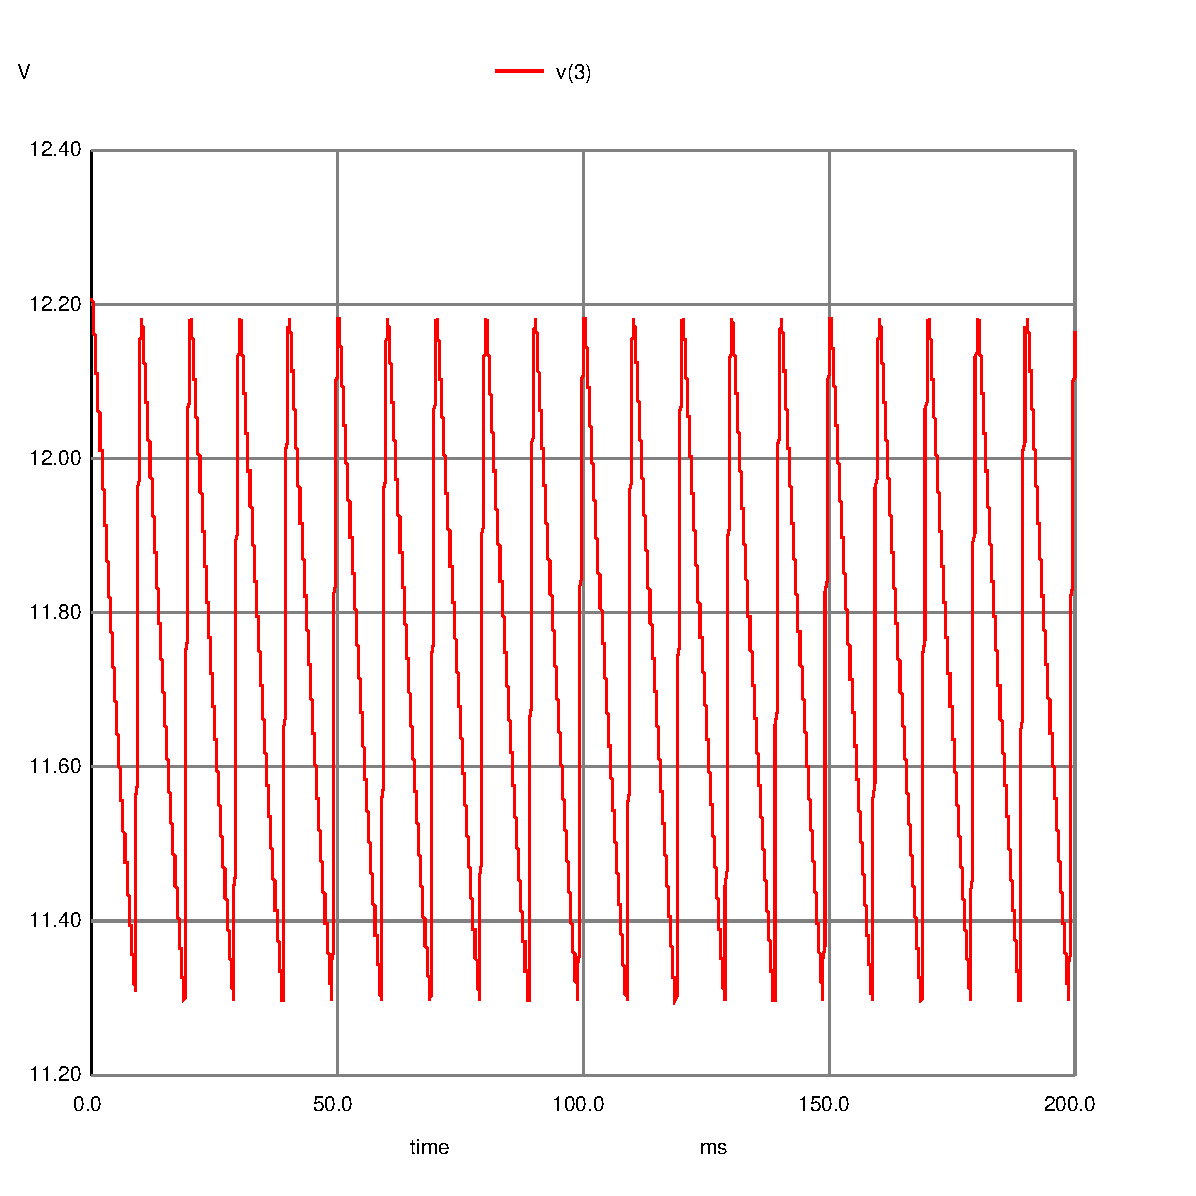
\includegraphics[width=0.6\linewidth]{v_3.eps}
    \caption{Voltage after the envelope detector}
    \label{plot5}
\end{figure}

\begin{figure}[h]
    \centering
    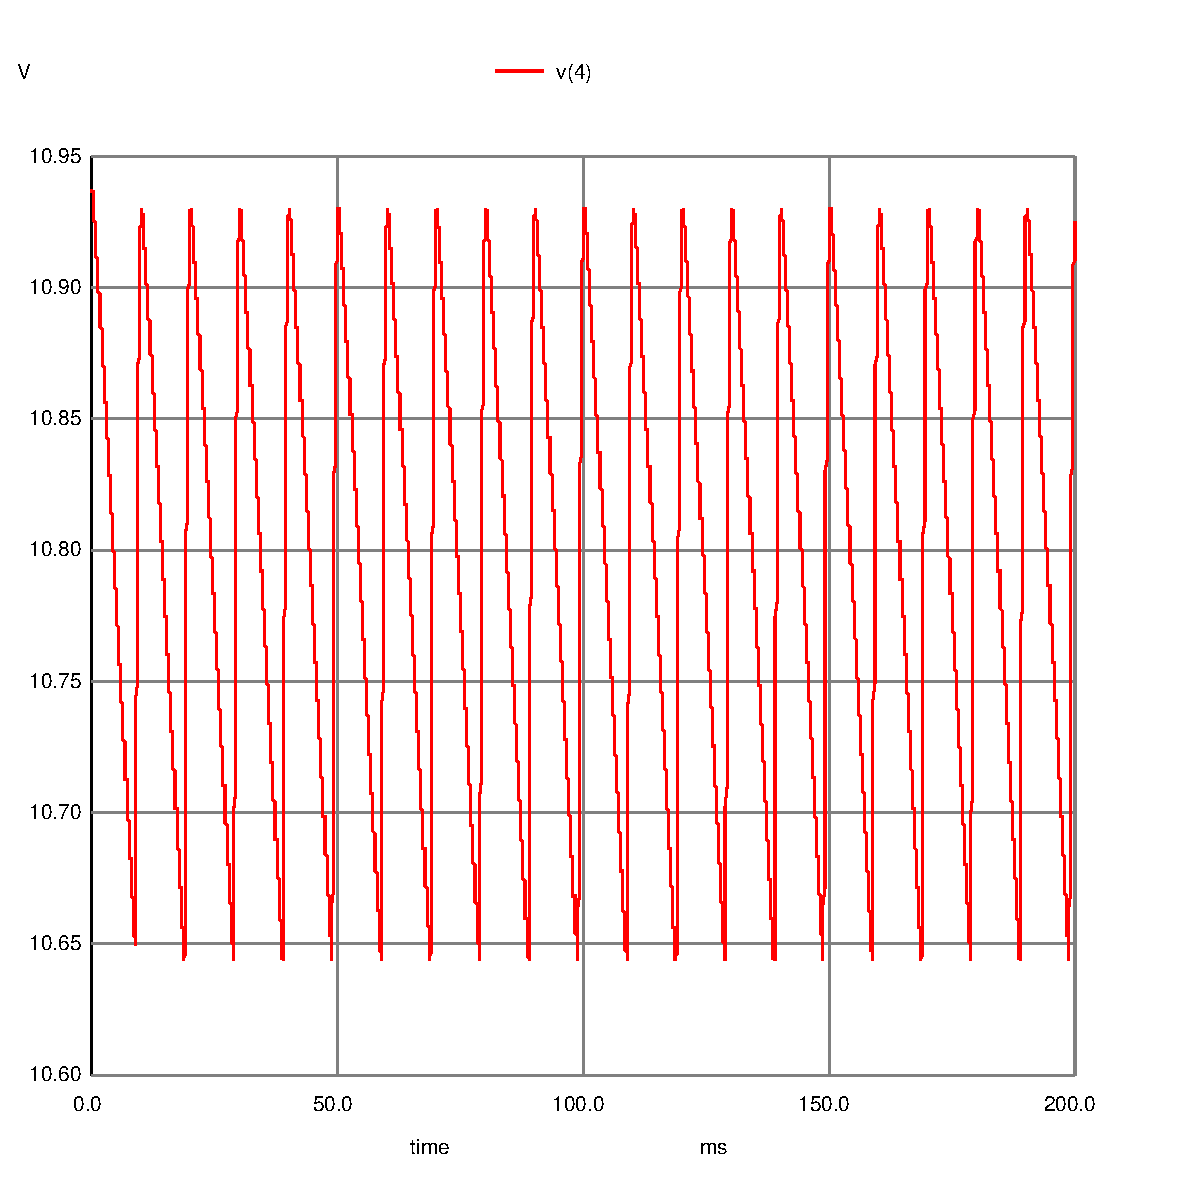
\includegraphics[width=0.6\linewidth]{v_4.eps}
    \caption{Voltage after the regulator}
    \label{plot6}
\end{figure}

\begin{figure}[h]
\centering
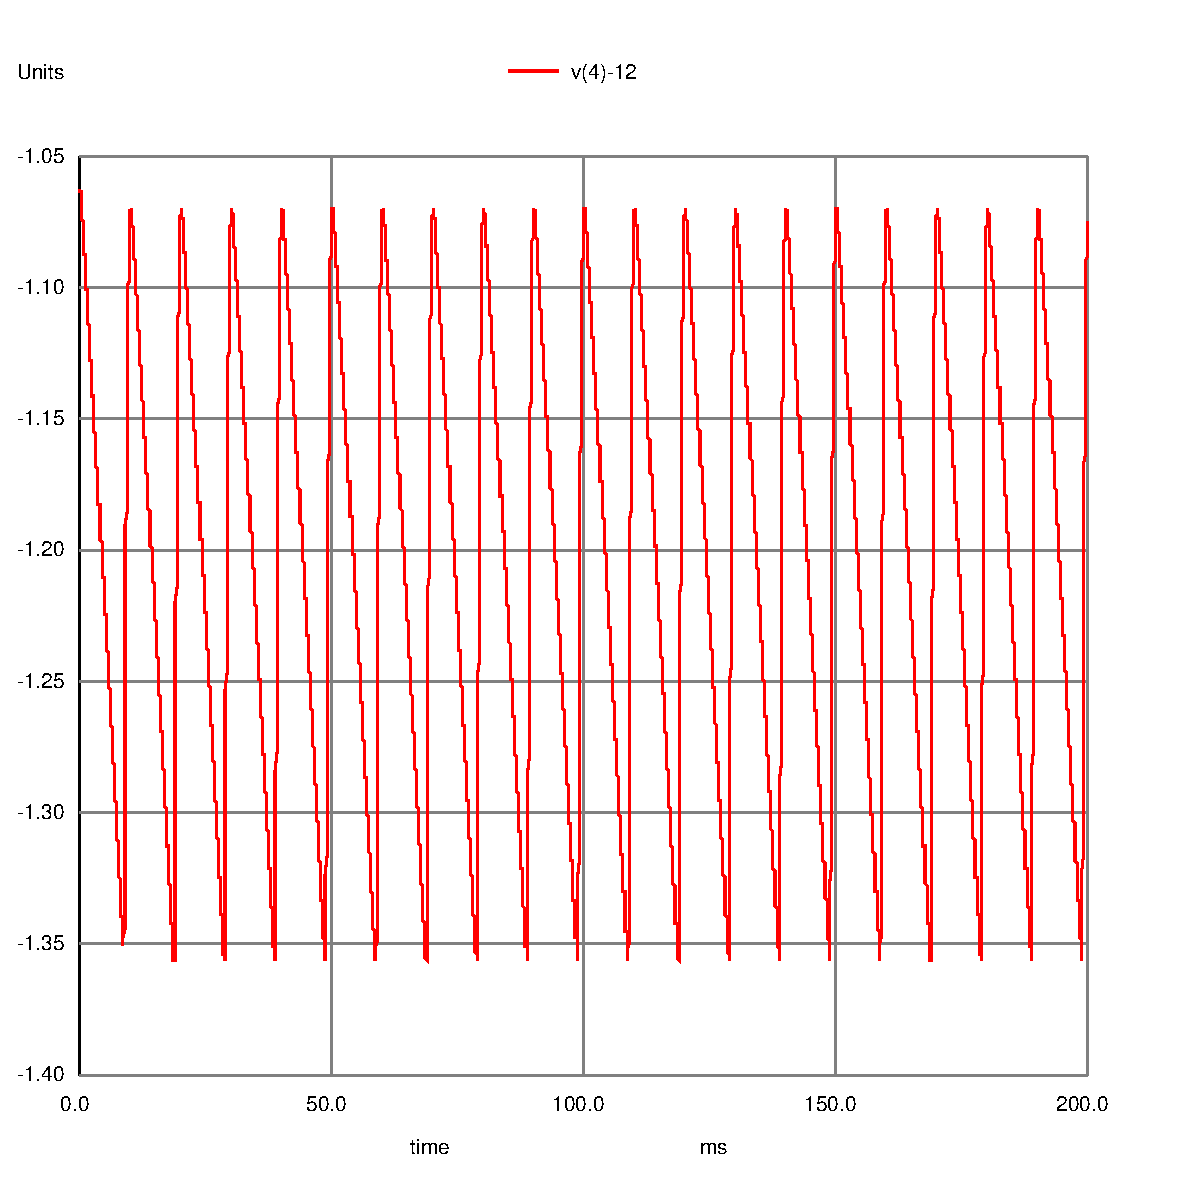
\includegraphics[width=0.6\linewidth]{delta_v.eps}
\caption{Voltage difference between the regulator output and the 12 V DC}
\label{plot7}
\end{figure}

\clearpage

The output voltage ripple and the DC level were simulated aswell and are as follows.

\begin{equation}
    V_{Ripple} = 0.2933 V
\end{equation}
\begin{equation}
    DC Level = 10.798
\end{equation}


\subsection{Comparisons}
\label{subsec:compare}

%In this last subsection, we present the values and plots obtained from the Theoretical Analysis and the Simulation Analysis that refer to the same sets of evaluations, for visualization purposes, and comment on their similarities or discrepancies.



All in all, there is an obvious difference between the theoretical and simulation results. The results obtained using \textit{Octave} are closer to the aimed values and oscillate less. The values obtained with \textit{Ngspice} are smaller ($v_4(t)$ is closer to 11V, for example). Nevertheless, the overall wave forms are similar, the frequency of the signals is the same, and, by both approaches, the results are satisfyingly accurate. 
The discrepancies stem from the different considerations made in the theoretical model and in the Ngspice software's models. In the Ngspice models, the approximations used when diodes are involved are much more complex and accurate.


\section{Conclusion}
\label{sec:conclusion}

In this laboratory assignment the objective of analysing an RC circuit has been
achieved. Static, time and frequency analyses have been performed both
theoretically using the Octave maths tool and by circuit simulation using the
Ngspice tool. The simulation results matched the theoretical results
precisely. The reason for this perfect match is the fact that this is a
straightforward circuit containing only linear components, so the theoretical


%\cleardoublepage

% ----------------------------------------------------------------------
%  Bibliography
% ----------------------------------------------------------------------
%\addcontentsline{toc}{section}{\bibname}
%\bibliographystyle{abbrvunsrtnat} % <<<<< SELECT IF USING REFERENCES BY NUMBER (CITATION ORDER)
%\bibliography{../../../BIBfile.bib}

% ----------------------------------------------------------------------
\end{document}
% ----------------------------------------------------------------------

